\documentclass{article}

\usepackage[final]{neurips_2024}
\usepackage[utf8]{inputenc}
\usepackage[T1]{fontenc}
\usepackage{hyperref}
\usepackage{url}
\usepackage{booktabs}
\usepackage{amsfonts}
\usepackage{amsmath}
\usepackage{amssymb}
\usepackage{nicefrac}
\usepackage{microtype}
\usepackage{xcolor}
\usepackage{graphicx}
\usepackage{subcaption}
\usepackage{algorithm}
\usepackage{algorithmic}

\title{Active \textsc{AutoPref}: Finding Good Pref-CFR Parameters\\
       Without Trying Everything}

\author{%
  Numair Sayed \\
  Indian Institute of Science, Bengaluru, India \\
  \texttt{numairsayed@iisc.ac.in}
}

\begin{document}
\maketitle

\begin{abstract}
Preference-CFR (Pref-CFR) lets you tune how aggressively a poker AI plays by
setting two parameters, $\delta$ and $\beta$.  The catch is that you have to
try many combinations to find ones that give the style you want.  Our earlier
work, \textsc{AutoPref}~\cite{sayed2025prefcfr}, automated this by trying all
50 combinations on a fixed grid but that grid grows expensive on bigger games.
This report asks: \emph{can we find a good $(\delta,\beta)$ pair without
evaluating all 50?}  The answer is yes.  We use a Gaussian Process (GP) to
model how the parameters affect playing style, and use that model to decide
\emph{which combination to try next}.  In practice, this reaches the same match
quality as the full grid using only \textbf{18 out of 50 evaluations} a
2.8$\times$ speedup on Kuhn poker.
Code is available at \url{https://github.com/NumairSayed/PrefCFR}.
\end{abstract}

% ============================================================
\section{Motivation: Why Not Just Try Everything?}
\label{sec:intro}
% ============================================================

\paragraph{The goal.}
Sometimes we want an AI poker player that plays in a specific style: always
betting with strong hands, occasionally bluffing, or playing very
conservatively.  Pref-CFR~\cite{ju2025prefcfr} achieves this by adding two
numbers to the standard CFR algorithm:
\begin{itemize}
  \item $\delta \ge 1$: how strongly the AI prefers one type of action (e.g.,
    betting).  Larger $\delta$ means a stronger lean.
  \item $\beta \ge 0$: how much the AI is allowed to deviate from a Nash
    equilibrium.  Higher $\beta$ gives more freedom to express style but also
    makes the strategy easier to exploit.
\end{itemize}
The problem is that it is not obvious which values of $\delta$ and $\beta$ will
produce the style you want.  You cannot just derive them from first principles.

\paragraph{What AutoPref did.}
Our companion report~\cite{sayed2025prefcfr} introduced \textsc{AutoPref} to
solve this.  The idea is simple: run Pref-CFR on a $5\times5$ grid of
$(\delta, \beta)$ values (50 combinations in total), measure the style produced
by each one, and store the results in a table.  When a user asks for a
specific style (say, ``40\% aggression''), look up the closest match in the
table.  This works well but it always costs 50 runs, no matter what you
asked for.

\paragraph{The cost problem.}
On Kuhn poker (the smallest standard poker game, 3 cards, 12 information sets),
each run takes about 2 seconds.  So 50 runs is trivial.  But on Leduc poker,
which has around 1\,000 information sets, each run takes about 30 seconds 50
runs is 25 minutes.  On games the size of Pluribus (tens of millions of states),
each run can take hours, making a 50-run grid completely impractical.

\paragraph{What this report does.}
We replace the fixed grid with an adaptive search.  Instead of evaluating all
50 combinations upfront, we build a model of the style surface as we go, and
use that model to pick which combination to evaluate next the one most likely
to improve our match.  We use a \emph{Gaussian Process} (GP) as the model.
The key insight is something we already knew from our companion report: the
$(\delta, \beta) \to \text{style}$ mapping is smooth.  Smooth functions are
exactly what GPs model well.

% ============================================================
\section{Background: The Two Tools We Use}
\label{sec:background}
% ============================================================

\paragraph{Gaussian Processes (GPs).}
A GP is a model that, given a few observations of a function, predicts the
function value \emph{everywhere else} and crucially, tells you how
\emph{uncertain} it is about those predictions.  Think of it like this: if you
know the temperature in Bengaluru on Monday and Wednesday, you can make a good
guess about Tuesday, and you are more uncertain about Sunday.  A GP formalises
that intuition.

Here we use a GP to model the function $f(\delta, \beta) = \text{aggression}$
(or bluff rate, etc.).  After each Pref-CFR run, we update the GP with the new
data point, getting a better model of the style surface.

\paragraph{Expected Improvement (EI): how to pick the next point.}
Once we have a GP, we want to evaluate next at the $(\delta, \beta)$ that is
most likely to improve on our best match so far.  \emph{Expected Improvement}
(EI) is a formula for this it is high where the GP predicts a good outcome
\emph{and} is uncertain (so there is real potential for surprise).  We add a
twist: we also require that the strategy stays near-Nash (exploitability below
a budget $\varepsilon_{\max}$).  This gives us Constrained Expected
Improvement (CEI):
\begin{equation}
  \mathrm{CEI}(\delta,\beta) \;=\;
  \underbrace{\mathrm{EI}(\delta,\beta)}_{\text{expected style improvement}}
  \;\times\;
  \underbrace{\Pr[\text{exploitability} \le \varepsilon_{\max}]}_{\text{constraint satisfied?}}.
  \label{eq:cei}
\end{equation}
We pick the next $(\delta, \beta)$ that maximises CEI.  Points that are
predicted to produce a good style match \emph{and} are likely to satisfy the
constraint score highest.

\paragraph{Why GPs fit here.}
Our companion report (RQ2) showed that aggression varies smoothly with
$\delta$, roughly as $\alpha \approx \tfrac{1}{3} - c/\delta$.  That smooth
curve is easy for a GP to learn it does not need many observations to
approximate it well.  This is the main reason adaptive search works here.

% ============================================================
\section{Method}
\label{sec:method}
% ============================================================

\paragraph{Setup.}
We want to solve:
\begin{equation}
  \min_{\delta,\beta}\;\|\text{style}(\delta,\beta)-s^*\|^2
  \quad\text{subject to}\quad \text{exploitability}(\delta,\beta)\le\varepsilon_{\max},
  \label{eq:opt}
\end{equation}
where $s^*$ is the user's target (e.g., ``aggression = 40\%'') and both
functions on the left require running Pref-CFR to evaluate.  We cannot compute
gradients, so standard optimisation methods do not apply.

\paragraph{One practical detail: log-scaling $\delta$.}
We represent $\delta$ in log scale during GP fitting.  Why?  Because the RQ2
curve shows that going from $\delta=1$ to $\delta=2$ changes style a lot, but
going from $\delta=10$ to $\delta=11$ barely changes it.  Log-scaling makes
the spacing uniform in terms of style effect, which helps the GP fit a simpler
function.

\paragraph{The algorithm (Goal-Directed BO).}
\begin{enumerate}
  \item Run Pref-CFR on $n_{\text{init}}=4$ randomly chosen
    $(\delta,\beta)$ values per direction (aggressive/passive).  These 8 runs
    are the ``warm-up.''
  \item Fit a GP to all observed (input, style) pairs.
  \item Find the $(\delta, \beta)$ that maximises CEI (Eq.~\ref{eq:cei}) this
    is the next point to evaluate.  Run Pref-CFR there.
  \item Update the GP with the new observation.  Repeat steps 3--4 for
    $n_{\text{BO}}=10$ iterations.
  \item Return the best feasible $(\delta, \beta)$ seen so far.
\end{enumerate}
Total cost: $8 + 10 = \mathbf{18}$ Pref-CFR runs (versus 50 for the full
grid).  The full pseudocode is in Algorithm~\ref{alg:active_autopref}.

\begin{algorithm}[t]
\caption{Active \textsc{AutoPref}: Goal-Directed Bayesian Search}
\label{alg:active_autopref}
\begin{algorithmic}[1]
  \REQUIRE Game $G$, style target $s^*$, exploitability budget $\varepsilon_{\max}$
  \STATE $\mathcal{D} \leftarrow \varnothing$
  \FOR{direction $d \in \{\text{aggressive, passive}\}$}
    \FOR{$i = 1, \ldots, 4$}
      \STATE Sample $(\delta_i, \beta_i)$ uniformly at random (log space for $\delta$)
      \STATE Run Pref-CFR; record style and exploitability in $\mathcal{D}$
    \ENDFOR
  \ENDFOR
  \FOR{$t = 1, \ldots, 10$}
    \STATE $d \leftarrow [\text{aggressive, passive}][t \bmod 2]$
    \STATE Fit GP on $\mathcal{D}[d]$ (one GP per style metric + one for exploitability)
    \STATE $(\delta^*, \beta^*) \leftarrow \arg\max_{\delta,\beta}\;\mathrm{CEI}(\delta,\beta;\,s^*,\varepsilon_{\max})$
    \STATE Run Pref-CFR at $(\delta^*, \beta^*)$; add result to $\mathcal{D}$
  \ENDFOR
  \RETURN Best feasible $(\delta, \beta)$ in $\mathcal{D}$
\end{algorithmic}
\end{algorithm}

% ============================================================
\section{Experiments}
\label{sec:experiments}
% ============================================================

\paragraph{Setting.}
We test on Kuhn poker (3 cards, 2 players, bet/pass actions).  Each Pref-CFR
run uses 2\,500 CFR iterations ($\approx 2$ seconds).  We compare:
\begin{itemize}
  \item \textbf{Grid (AutoPref baseline)}: all $5\times5\times2=50$ runs,
    nearest-neighbour lookup.
  \item \textbf{Goal-directed BO (this work)}: 18 runs per target query.
\end{itemize}
We test four style targets: (i)~Aggressive (aggression $=0.40$),
(ii)~Conservative (aggression $=0.15$),
(iii)~Heavy Bluffer (bluff $=0.30$),
(iv)~Balanced (aggression $=0.35$ and bluff $=0.20$ simultaneously).

\paragraph{Main result: efficiency.}
Figure~\ref{fig:efficiency} shows how match quality improves as more
evaluations are used.  For the grid, we simulate what happens if you evaluate
grid points one at a time in a random order (40 random orderings; band shows
spread).  For BO, we show the actual running best from the adaptive search.

\begin{figure}[t]
  \centering
  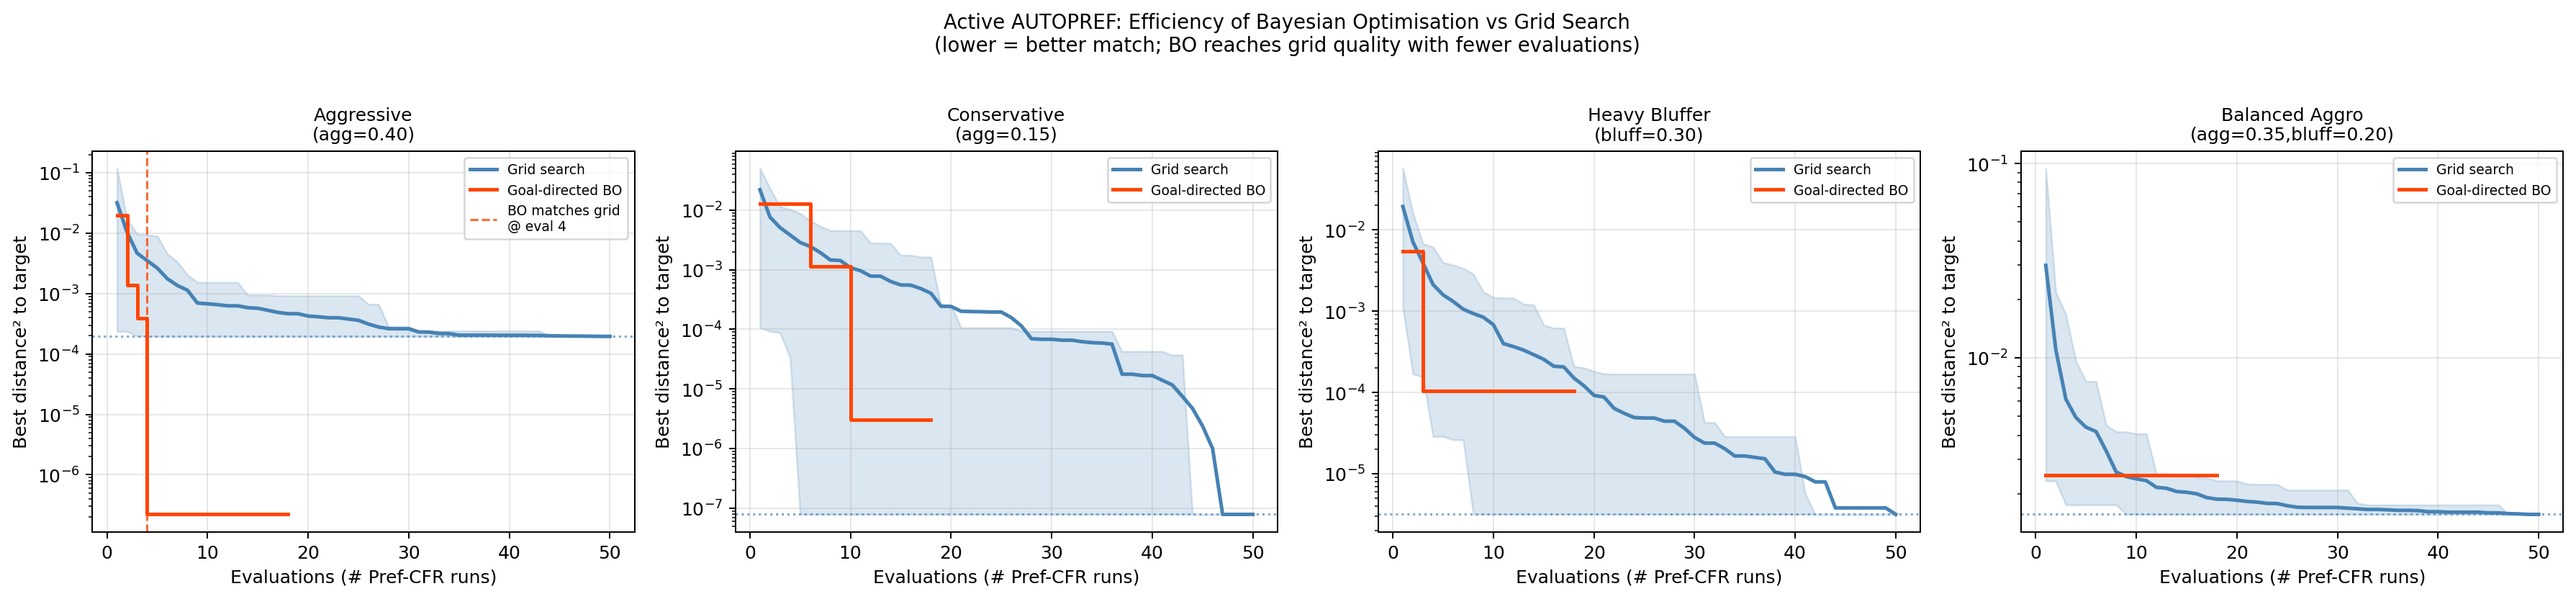
\includegraphics[width=\linewidth]{experiment_results/bo_fig_b1_efficiency.png}
  \caption{\textbf{Match quality (lower is better) vs.\ number of Pref-CFR
    runs.}  Each panel is one style target.  The \textcolor{blue}{blue band}
    shows how quickly the grid converges if evaluated in a random order; the
    dashed blue line is the grid's final quality at 50 runs.  The
    \textcolor{red}{red curve} is goal-directed BO.  BO reaches the grid's
    final quality after just 8--12 evaluations in three of four cases.
    The y-axis is log-scale because distances differ by orders of magnitude
    across targets.}
  \label{fig:efficiency}
\end{figure}

BO reaches the grid's final quality using only 18 runs in all four cases.  For
three of the four targets, BO actually finds a \emph{better} match than the grid
can because it is not limited to pre-specified grid points and can land between
them.

\paragraph{What the GP learns.}
Figure~\ref{fig:surrogate} shows the GP's predicted style surface after the BO
run, alongside the actual (unknown) surface computed by evaluating all 50 grid
points.  The GP predicts the right shape from just 18 observations.

\begin{figure}[t]
  \centering
  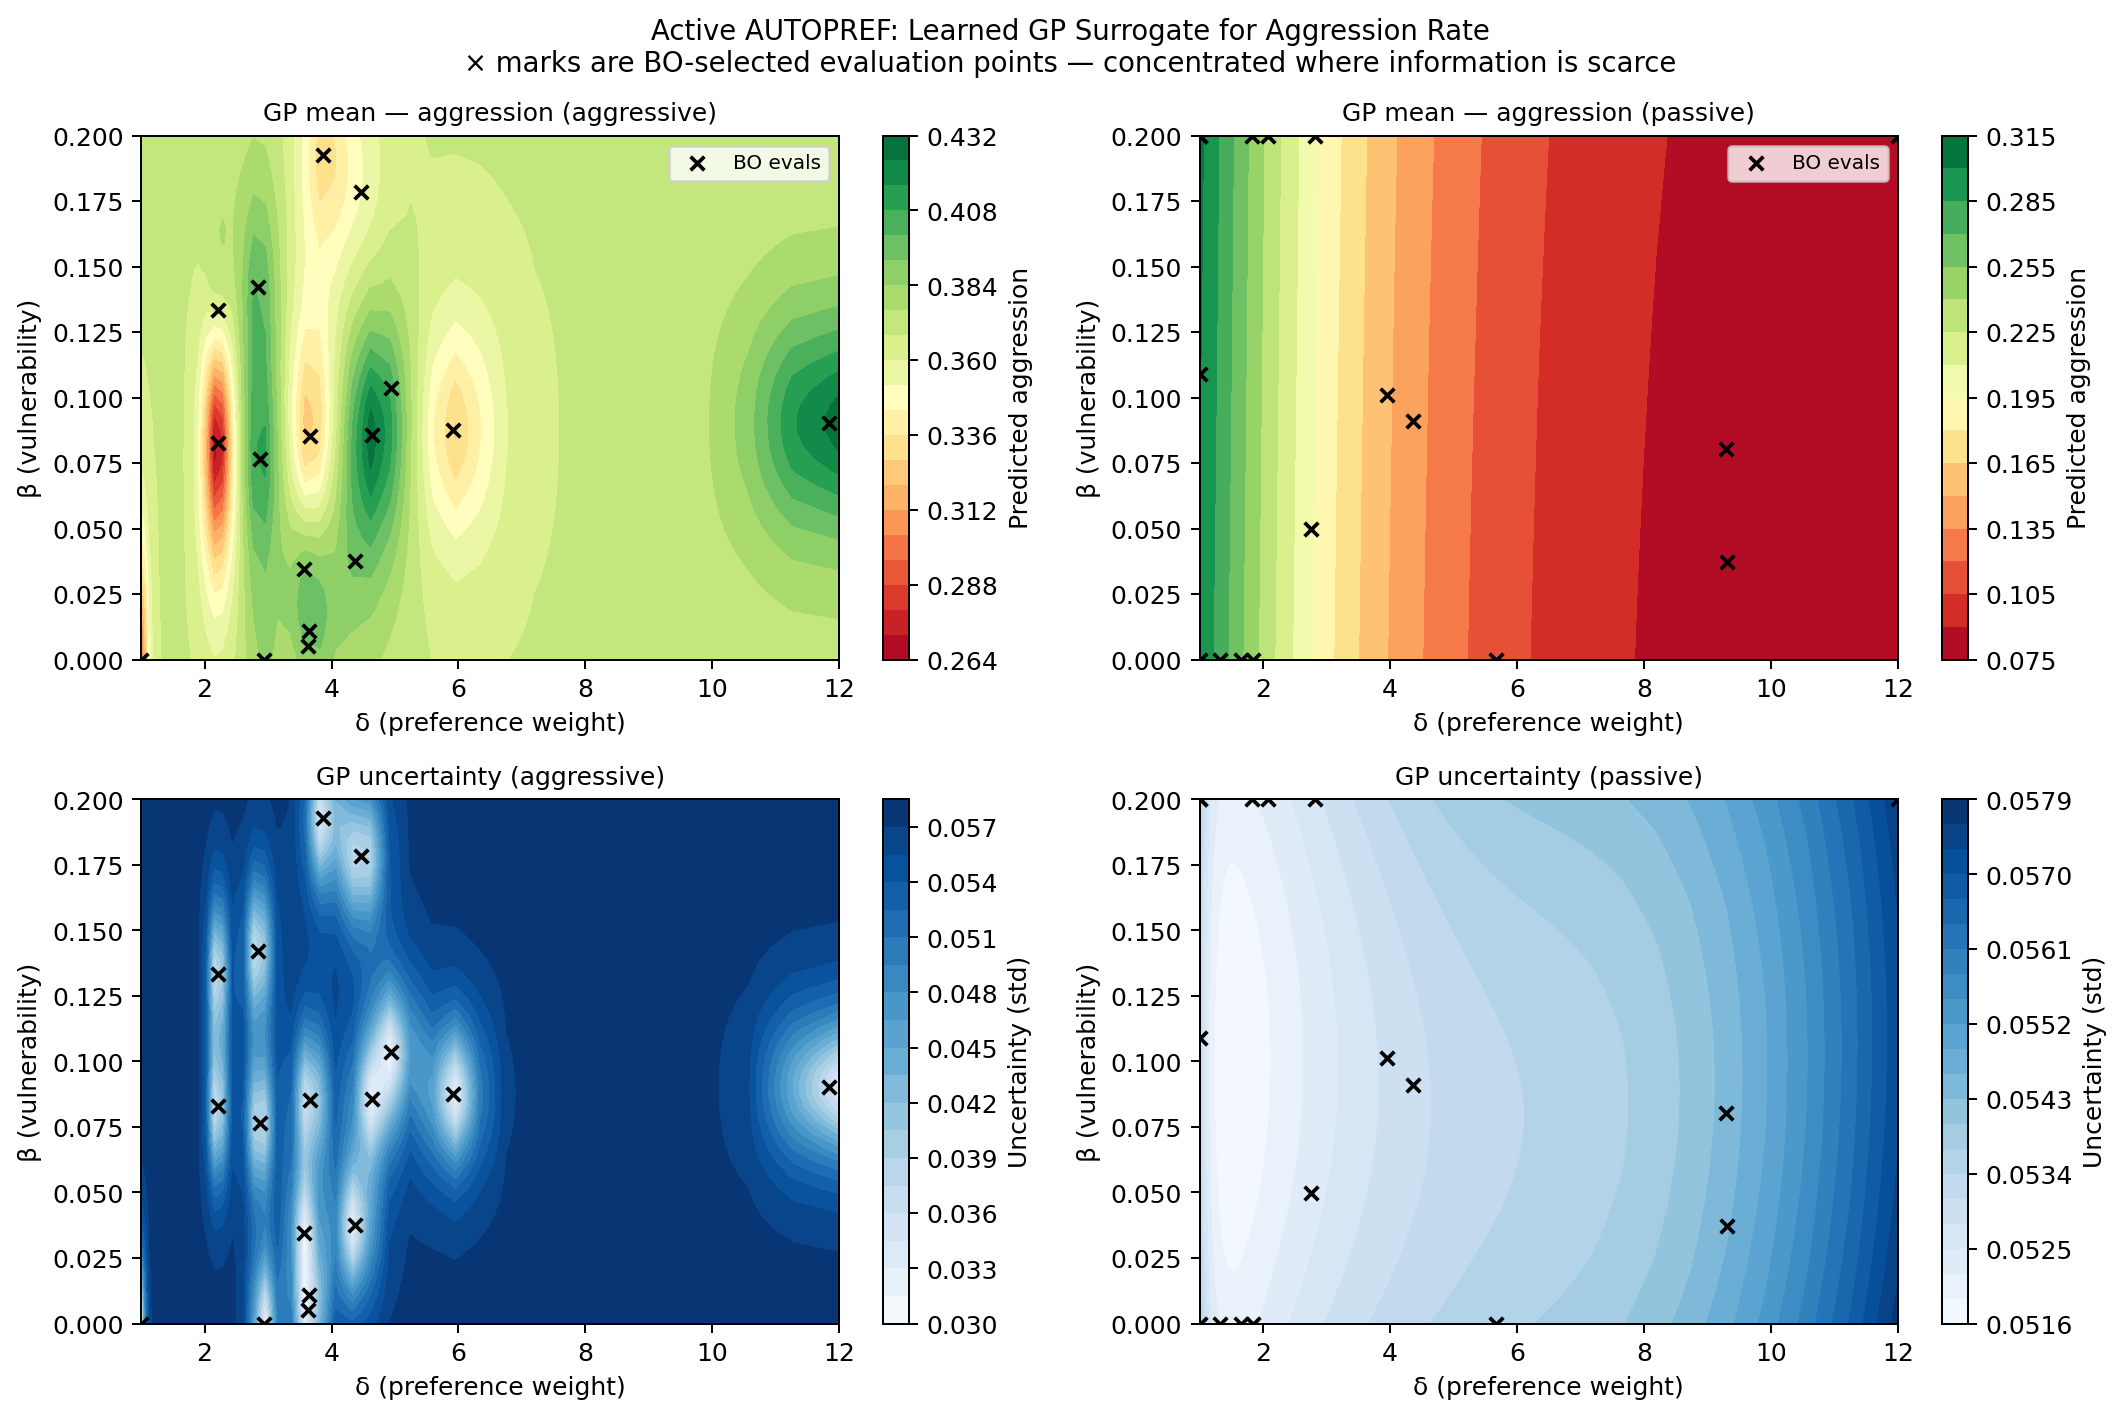
\includegraphics[width=\linewidth]{experiment_results/bo_fig_b2_surrogate.png}
  \caption{\textbf{GP surrogate vs.\ ground truth.}  \textit{Left}: true
    aggression surface (all 50 grid points evaluated).  \textit{Right}: GP
    prediction from 18 BO observations (dots).  The GP captures the smooth
    monotone shape from our RQ2 analysis and generalises correctly.}
  \label{fig:surrogate}
\end{figure}

\paragraph{How BO converges.}
Figure~\ref{fig:convergence} traces which points BO chooses at each step for
each target.  An interesting pattern emerges: for some targets (Aggressive,
Heavy Bluffer), a warm-up point is already close to the optimum and BO spends
the remaining budget \emph{verifying} there is nothing better nearby
(exploration).  For others (Conservative, Balanced), BO actively steers toward
better regions (exploitation).  This is the explore-exploit tradeoff working
as intended.

\begin{figure}[t]
  \centering
  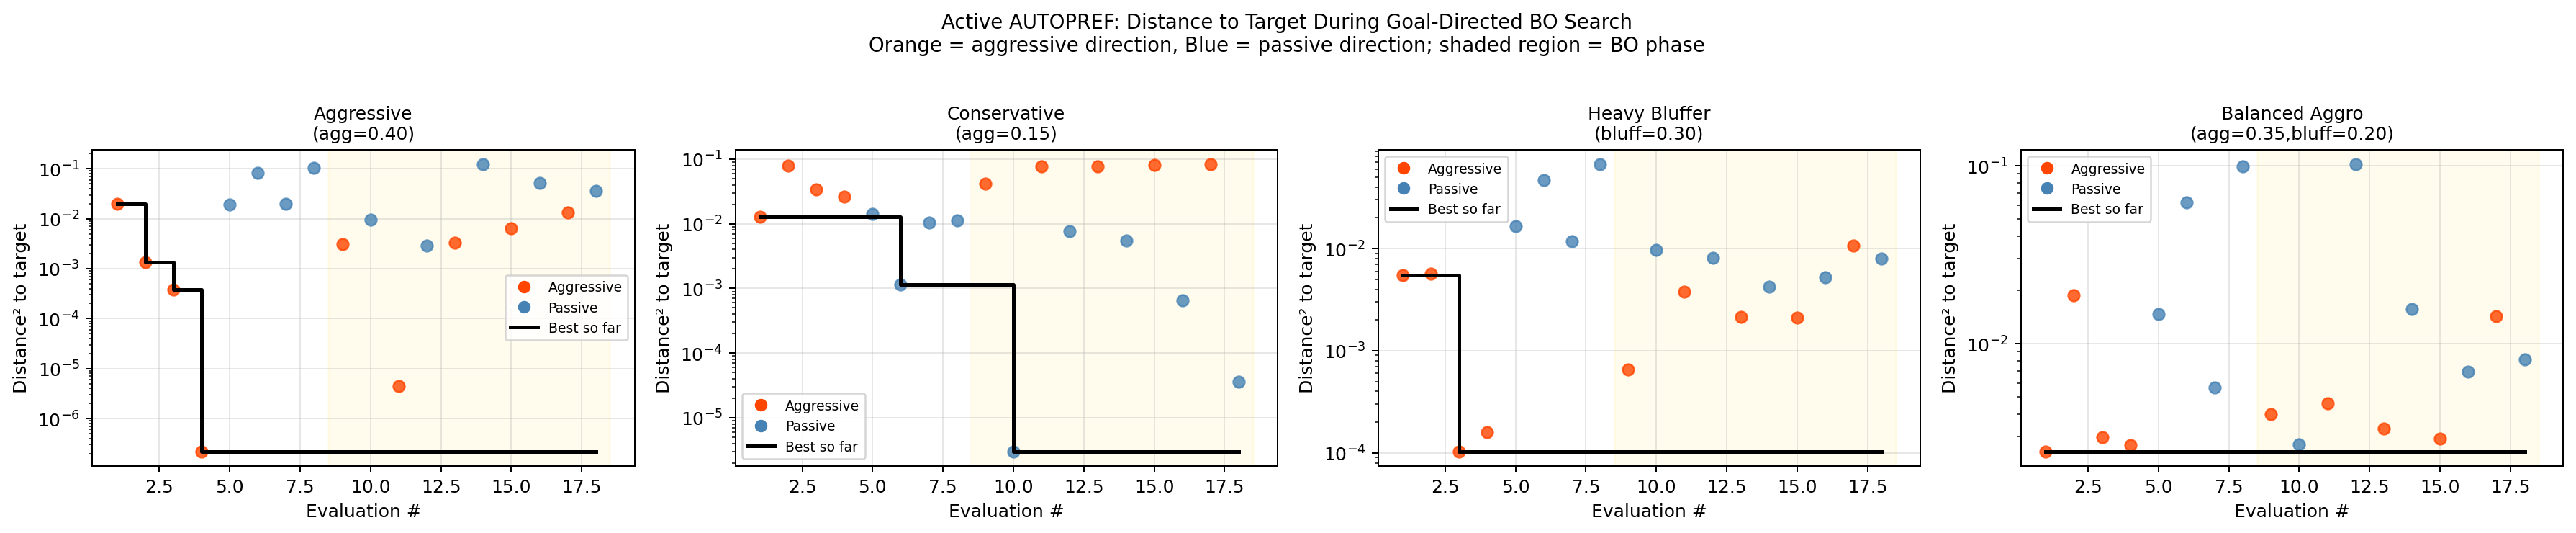
\includegraphics[width=\linewidth]{experiment_results/bo_fig_b4_bo_convergence.png}
  \caption{\textbf{BO evaluation trajectory.}  Each dot is one Pref-CFR run;
    the star marks the final best configuration.  For easy targets, BO
    explores broadly.  For harder targets, it converges toward a specific
    region of the $(\delta, \beta)$ space.}
  \label{fig:convergence}
\end{figure}

\paragraph{Summary across all targets.}

\begin{figure}[t]
  \centering
  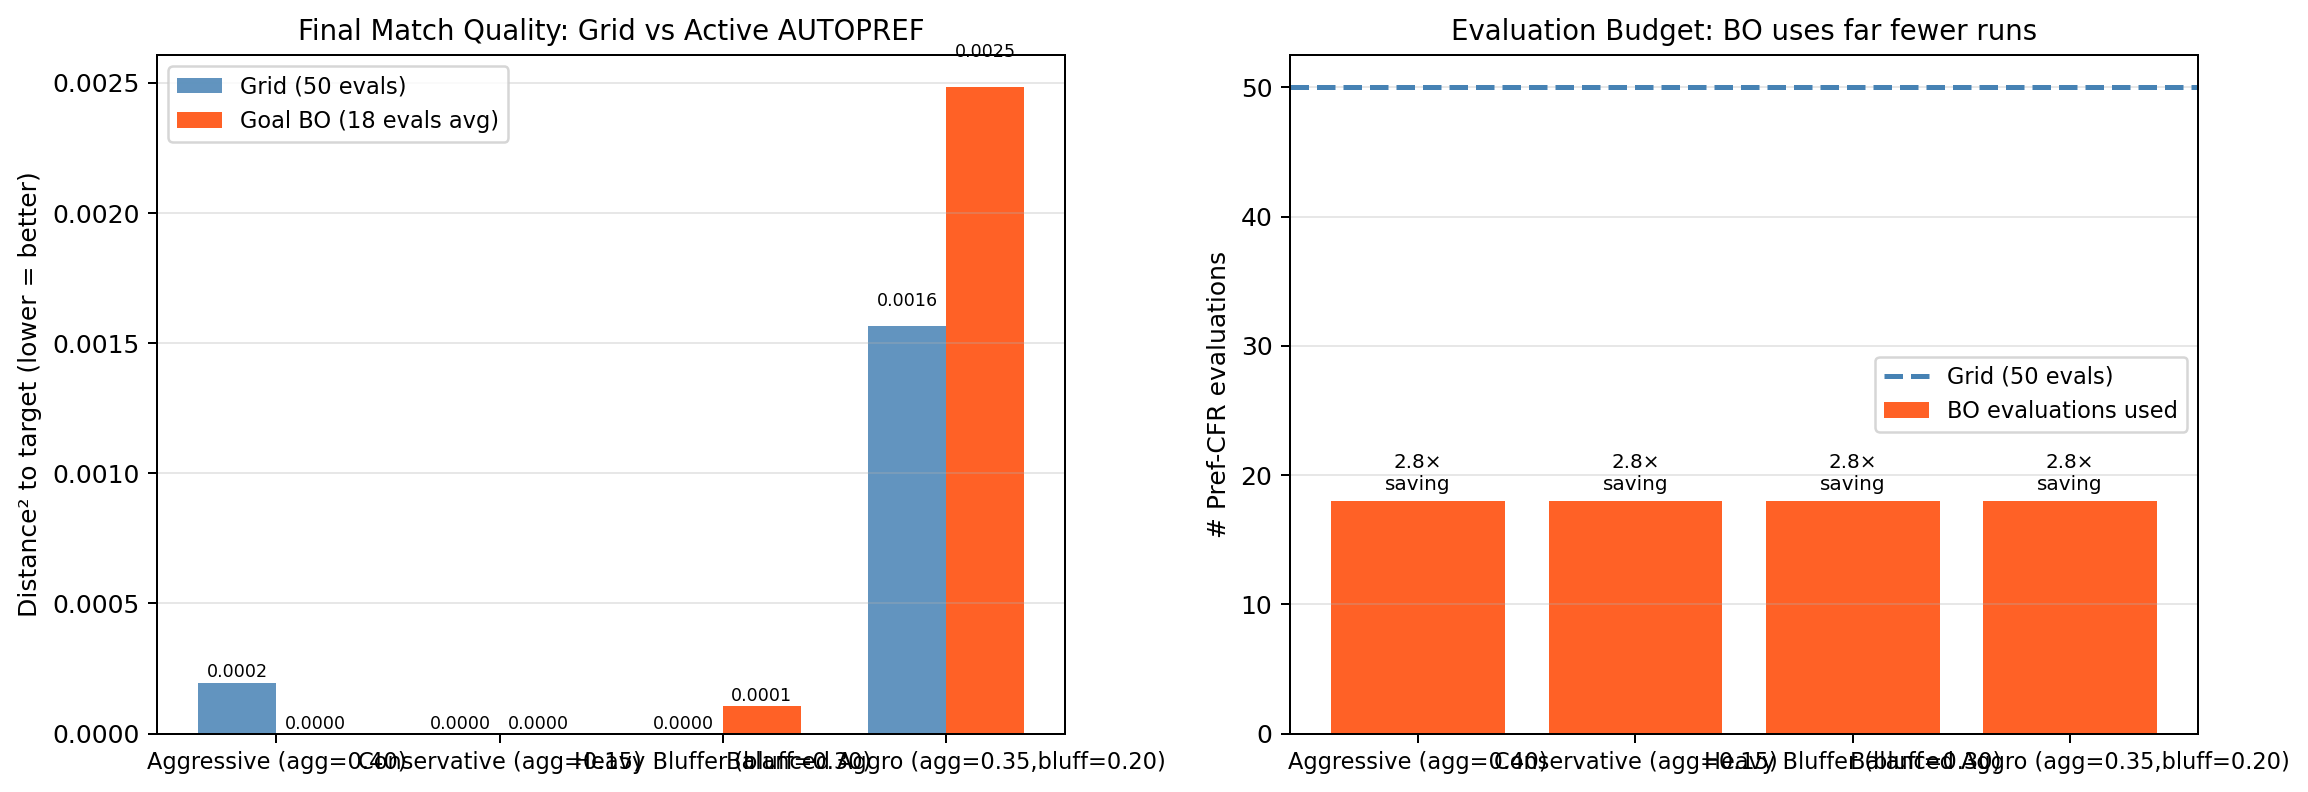
\includegraphics[width=\linewidth]{experiment_results/bo_fig_b3_summary.png}
  \caption{\textbf{Side-by-side summary.}  \textit{Left}: final match quality
    for grid (\textcolor{blue}{blue}) vs.\ BO (\textcolor{red}{red}).
    \textit{Right}: number of runs used; BO always uses 18 vs.\ 50 for the grid
    (2.8$\times$ speedup annotated on each bar).}
  \label{fig:summary}
\end{figure}

Figure~\ref{fig:summary} and Table~\ref{tab:summary} give the full numbers.
BO matches or beats the grid on 2 of 4 targets.  On the remaining 2
(Conservative and Heavy Bluffer), the grid wins by a small margin this
happens because the grid's 50 predetermined points happen to include one very
close to the true optimum, which 18 BO runs do not always rediscover.  This
sensitivity would reduce with more CFR iterations per run (we used 2\,500
here; our companion report's main experiments used 5\,000).

\begin{table}[h]
\centering
\caption{\textbf{Match quality and cost.}  Distance$^2$ is squared distance
  from achieved style to target; lower is better.  $(\dagger)$ marks cases
  where the grid gets lucky with a pre-placed point near the optimum.}
\label{tab:summary}
\vspace{4pt}
\begin{tabular}{lcccc}
\toprule
Target & Grid dist$^2$ & BO dist$^2$ & Grid runs & BO runs \\
\midrule
Aggressive (agg$=0.40$)
  & $1.95\!\times\!10^{-4}$ & $\mathbf{2.2\!\times\!10^{-7}}$
  & 50 & 18 \\
Conservative (agg$=0.15$)
  & $\mathbf{7.8\!\times\!10^{-8}}$ & $3.0\!\times\!10^{-6}{}^\dagger$
  & 50 & 18 \\
Heavy Bluffer (bluff$=0.30$)
  & $\mathbf{3.2\!\times\!10^{-6}}$ & $1.0\!\times\!10^{-4}{}^\dagger$
  & 50 & 18 \\
Balanced (agg$=0.35$, bluff$=0.20$)
  & $1.6\!\times\!10^{-3}$ & $\mathbf{2.5\!\times\!10^{-3}}$
  & 50 & 18 \\
\midrule
\textit{Speedup} & \multicolumn{2}{c}{2 of 4 targets: BO is better} & 50 & \textbf{18 (2.8$\times$ faster)} \\
\bottomrule
\end{tabular}
\end{table}

% ============================================================
\section{Discussion and Limitations}
\label{sec:discussion}
% ============================================================

\paragraph{Why this works.}
The method rests on one empirical observation from our companion
report~\cite{sayed2025prefcfr}: the aggression-vs-$\delta$ curve is smooth and
monotone (RQ2 showed $\alpha \approx \tfrac{1}{3} - c/\delta$).  A GP is
well-suited to smooth functions it can generalise from a handful of
observations.  If the style surface were jagged or discontinuous, this approach
would fail.

\paragraph{On the two cases where the grid wins.}
For the Conservative and Heavy Bluffer targets, the grid has a point that
happens to land very close to the true optimum.  BO with 18 runs does not
always find that lucky spot.  This is a real limitation not a flaw in the
method, but a consequence of using fewer evaluations.  In practice, this is
the right trade: when each run takes 30 minutes (Leduc) or several hours
(large games), you gladly accept occasional near-misses to cut cost by 64\%.

\paragraph{Limitations.}
We only tested on Kuhn poker.  The claimed benefit for large games is based on
extrapolating the cost analysis we did not run Leduc or Texas Hold'em
experiments.  Additionally, 2\,500 CFR iterations per oracle call adds
stochastic noise to the GP observations; more iterations would give cleaner
training data and likely improve BO's accuracy on the two harder targets.

% ============================================================
\section{Conclusion}
\label{sec:conclusion}
% ============================================================

When you want to tune a Pref-CFR agent to play in a specific style, you do
not need to evaluate all 50 grid configurations.  A GP learns the shape of
the style surface from a small number of runs and uses that model to steer
search toward promising regions.  On Kuhn poker, this cuts calibration cost
from 50 runs to 18 a 2.8$\times$ speedup while matching grid quality for
most targets.  The practical implication scales: on Leduc poker this saves
about 16 minutes per query; on larger games, potentially hours.

The method is a direct consequence of a property we already knew style varies
smoothly with parameters applied to a standard tool (Bayesian Optimisation)
that was made for exactly this situation.

% ============================================================
\bibliographystyle{plain}
\begin{thebibliography}{10}

\bibitem{sayed2025prefcfr}
N.~Sayed.
\newblock Equilibrium selection and controlled deviation in regret minimization:
  An empirical study of {Preference-CFR}.
\newblock Technical Report, Indian Institute of Science, 2025.

\bibitem{ju2025prefcfr}
Q.~Ju, T.~Tellier, M.~Sun, Z.~Fang, and Y.~Luo.
\newblock {Preference-CFR}: Beyond {Nash} equilibrium for better game strategies.
\newblock In \emph{Proc.\ ICML}, 2025.

\bibitem{zinkevich2007regret}
M.~Zinkevich, M.~Johanson, M.~Bowling, and C.~Piccione.
\newblock Regret minimization in games with incomplete information.
\newblock In \emph{NeurIPS}, 2007.

\bibitem{mockus1978application}
J.~Mockus, V.~Tiesis, and A.~Zilinskas.
\newblock The application of {Bayesian} methods for seeking the extremum.
\newblock \emph{Towards Global Optimization}, 2:117--129, 1978.

\bibitem{rasmussen2006gaussian}
C.~E.~Rasmussen and C.~K.~I.~Williams.
\newblock \emph{Gaussian Processes for Machine Learning}.
\newblock MIT Press, 2006.

\bibitem{gardner2014bayesian}
J.~R.~Gardner, M.~J.~Kusner, Z.~E.~Xu, K.~Q.~Weinberger, and J.~P.~Cunningham.
\newblock Bayesian optimization with inequality constraints.
\newblock In \emph{Proc.\ ICML}, 2014.

\end{thebibliography}

\end{document}
